\begin{exercice*}[Cercle]
    Soit un cercle $(\mathcal{C})$ de centre $O$.

    \begin{tikzpicture}[scale = 0.5]
        % \draw[help lines, color=black!30, dashed] (0,0) grid (10,10);        
        \coordinate[label=above:$O$] (O) at (5,5);
        \draw (4.9,5)--(5.1,5);
        \draw (5,4.9)--(5,5.1);
        \draw (O) circle (4);
    \end{tikzpicture}

    % \begin{multicols}2
        \begin{enumerate}
            \item Tracer deux diamètres $[AB]$ et $[CD]$ du cercle $(\mathcal{C})$.
            \item Justifier que les trianges $AOC$ et $BOD$ sont isométriques.
            \item Faire une déduction quant aux segments $[AC]$ et $[BD]$.
            \item Déterminer la nature du quadrilatère ainsi formé.
        \end{enumerate}
    % \end{multicols}
\end{exercice*}
\begin{corrige}
    %\setcounter{partie}{0} % Pour s'assurer que le compteur de \partie est à zéro dans les corrigés
    % \begin{multicols}2
        \begin{enumerate}
            \item \phantom{rrr}
            
                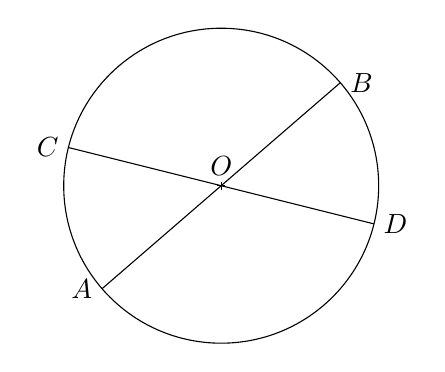
\begin{tikzpicture}[scale = 0.5]
                    % \draw[help lines, color=black!30, dashed] (0,0) grid (10,10);        
                    \coordinate[label=above:$O$] (O) at (5,5);
                    \draw (4.9,5)--(5.1,5);
                    \draw (5,4.9)--(5,5.1);
                    \draw (O) circle (4);
            
                    \coordinate[label=left:$A$] (A) at (1.97,2.38);
                    \coordinate[label=right:$B$] (B) at (8.03,7.62);
            
                    \draw (A)--(B);
            
                    \coordinate[label=left:$C$] (C) at (1.12,5.97);
                    \coordinate[label=right:$D$] (D) at (8.88,4.03);
            
                    \draw (C)--(D);
                \end{tikzpicture}

            \item Les angles $\widehat{AOC}$ et $\widehat{BOD}$ sont opposés par le sommet donc égaux.
            
            D'autre part, $OC=OD=OB=OA$ car $A$, $B$, $C$ et $D$ sont tous les quatre des points
            du cercle $(\mathcal{C})$ de centre $O$.

            Les triangles $AOC$ et $BOD$ ont un angle égal compris entre deux côtés égaux deux à deux.
            
            \psshadowbox{Ils sont donc isométriques}.
            \medskip
            \item Les triangles $AOC$ et $BOD$ sont iométriques donc $AC=BD$.
        \end{enumerate}
    % \end{multicols}
\end{corrige}

